\subsection{Command 2: pstree} 
\textbf{Purpose}
\begin{flushleft}
display a tree of processes
\end{flushleft}
\textbf{Usage}
\begin{verbatim}
pstree
pstree -c
pstree -p
\end{verbatim}
\textbf{Sample i/p and o/p}
\begin{figure}[H] 
\fbox{
\begin{minipage}{350px} 
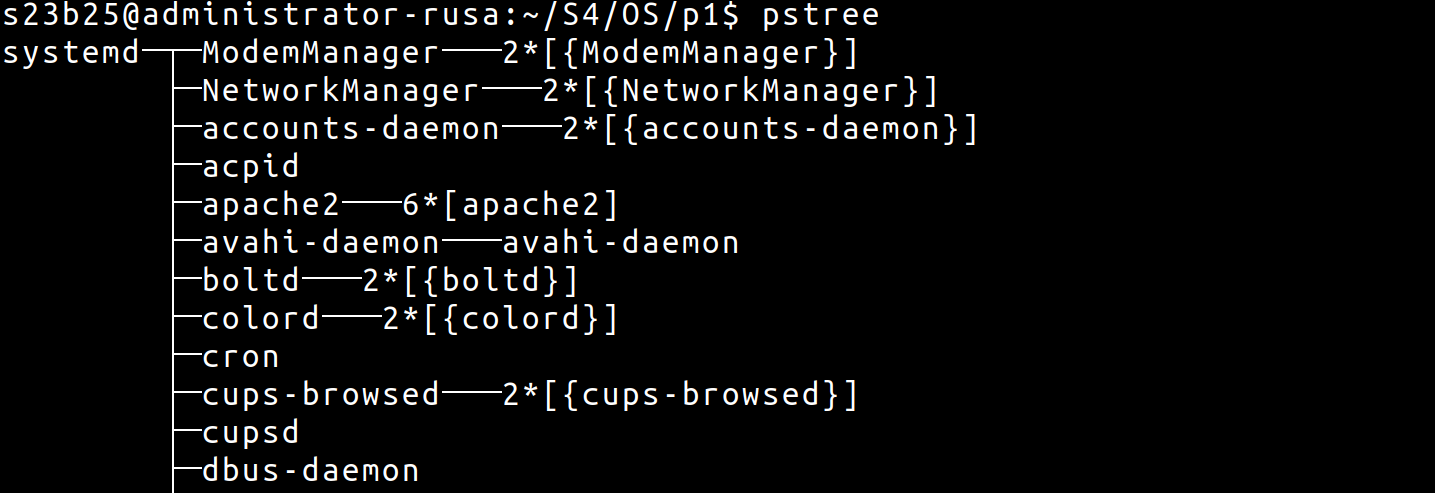
\includegraphics[width=\linewidth]{assets/pstree-1.png}
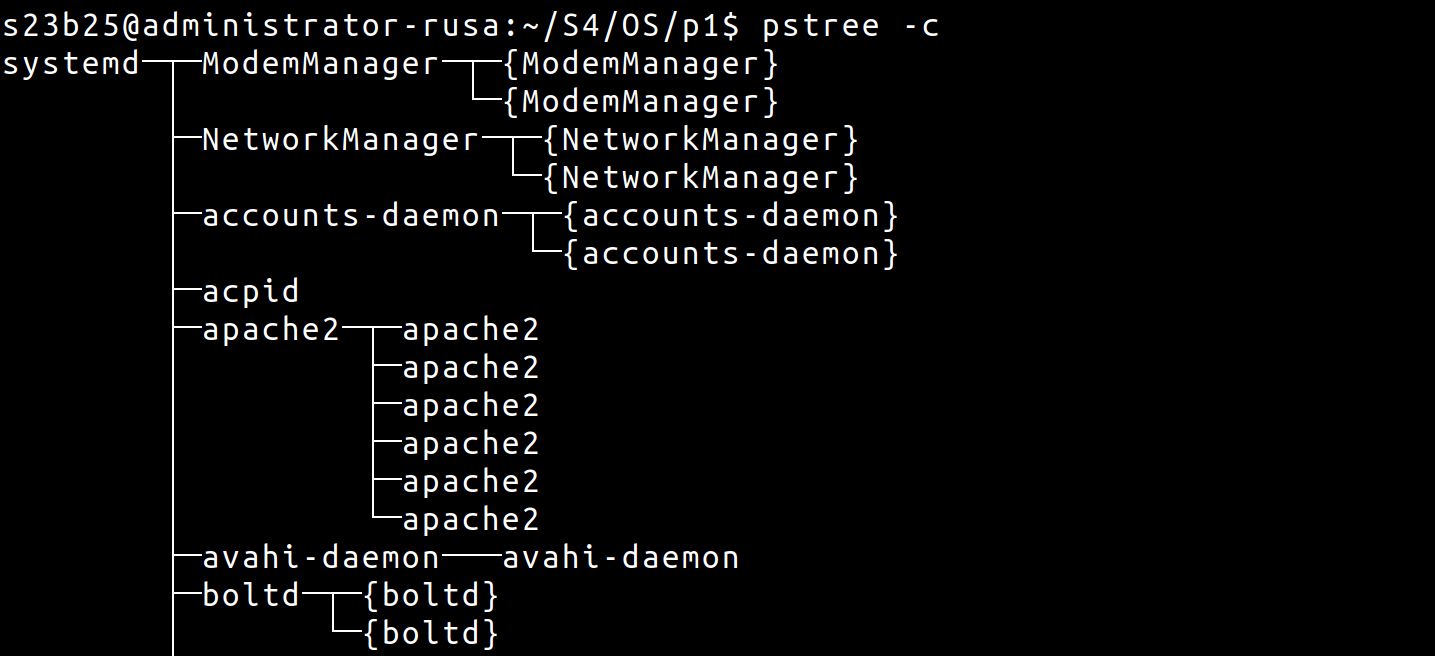
\includegraphics[width=\linewidth]{assets/pstree-2.png}
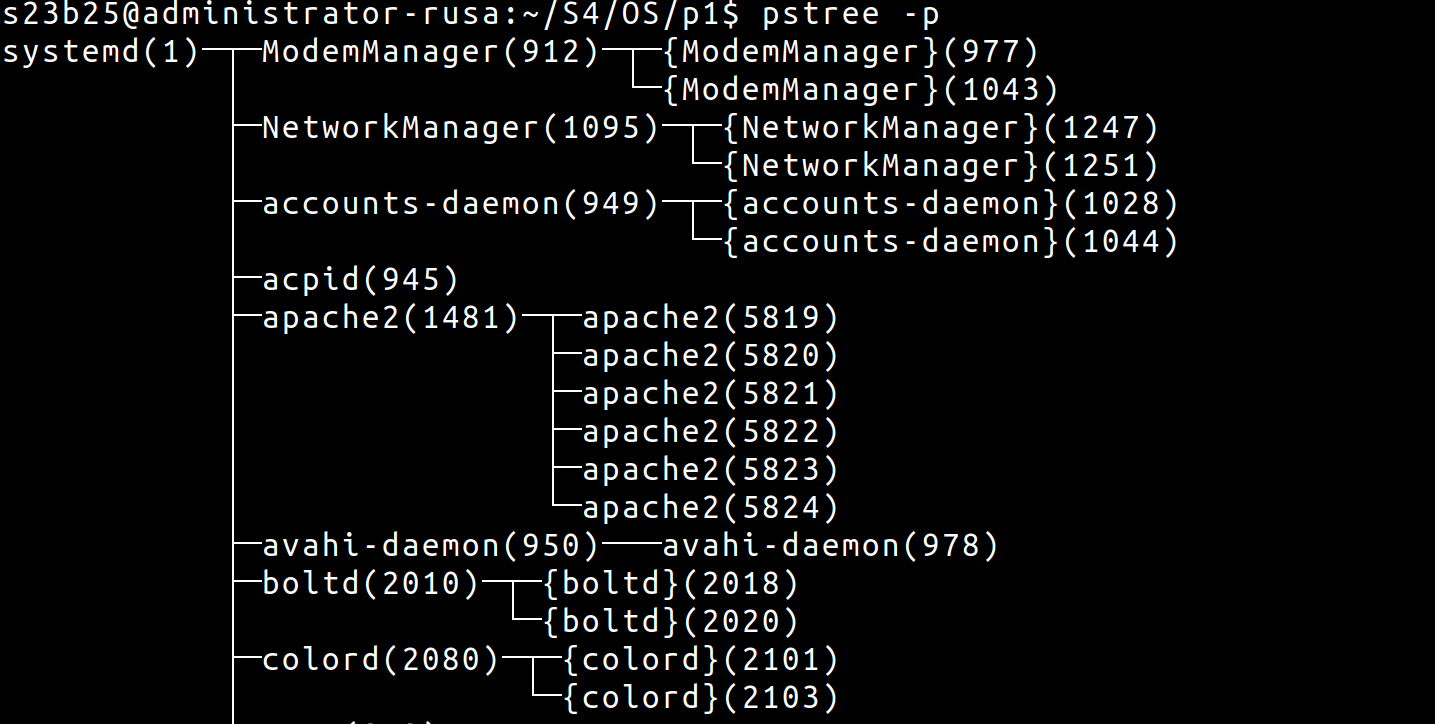
\includegraphics[width=\linewidth]{assets/pstree-3.png}
\end{minipage}
} %output screenshot name
\end{figure}
